\documentclass{standalone}
\usepackage[dvipsnames]{xcolor}
\usepackage{tikz}
%\usepackage{pgfplots}
%\usepackage{pgfplotstable}
%\pgfplotsset{compat=1.5}
\usetikzlibrary{patterns}
\tikzstyle{v par}=              [dash pattern=on 10pt off 5pt,color=red!70,line width = 2pt]
\tikzstyle{z direction}=      [dash pattern=on 10pt off 5pt on 2pt off 5pt, color=Blue,line width = 2pt]

\begin{document}
{
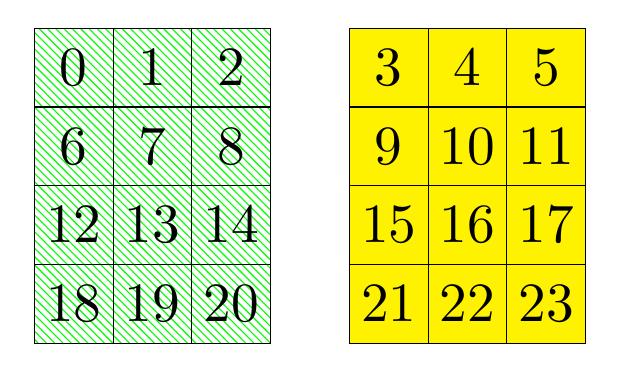
\begin{tikzpicture}
 
 \foreach \x in {0,...,2}
 {
  \foreach \y in {0,...,3}
  {
   \draw[pattern=north west lines, pattern color=green] (\x,\y) rectangle (\x+1,\y-1);
   \draw (\x,\y) -- (\x,\y-1) -- (\x+1,\y-1) -- (\x+1,\y) -- (\x,\y);
   \pgfmathsetmacro\n{int(\x+6*(3-\y))}
   \node[scale=2] at (\x+0.5,\y-0.5) {\n};
  }
 }
 
 \begin{scope}[xshift=1cm]
  
 \foreach \x in {3,...,5}
 {
  \foreach \y in {0,...,3}
  {
   \fill[color=yellow] (\x,\y) rectangle (\x+1,\y-1);
   \draw (\x,\y) -- (\x,\y-1) -- (\x+1,\y-1) -- (\x+1,\y) -- (\x,\y);
   \pgfmathsetmacro\n{int(\x+6*(3-\y))}
   \node[scale=2] at (\x+0.5,\y-0.5) {\n};
  }
 }
 \end{scope}

\end{tikzpicture}
}
\end{document}
